\section{The Architect's Question}\label{the-architects-question}

After this chapter we should be able to answer the inevitable scaling
question: \emph{a single GPU cannot hold this model or keep up with this
workload --- how do we split the work across many GPUs, and which split
is right?} We will build the arithmetic for why a model outgrows one
GPU, then study the five parallelization strategies --- tensor,
pipeline, data, expert, and sequence parallelism --- and develop a rule
for choosing among them based on the model's weight-residency, the
workload's batch shape, and the interconnect speed. After this chapter,
``we scaled it out'' becomes a precise claim about \emph{what} was split
and \emph{why}.

\section{Concept}\label{concept}

The central idea: parallelism is \textbf{splitting one of the three
things a model occupies --- its weights, its layers, or its data ---
across multiple devices.} Before reading on, one framing note that
prevents a common source of confusion: \textbf{the parallelism toolkit
differs between training and inference, and ``data parallelism'' means
different things in each mode.} In \emph{training}, DP means replicated
weights plus gradient all-reduce every step (plus FSDP, which shards and
re-gathers weights/optimizer state); the communication load is at the
gradient-sync point. In \emph{inference}, DP simply means running
independent model replicas to raise throughput --- there is no gradient
sync at all, because each request is served by one replica. There is
also an inference-specific family --- context/pipeline partitioning,
expert parallelism, and \textbf{P/D disaggregation} (splitting the
prefill stage from the decode stage into separate pools) --- which has
no training analogue. The rest of this section defines the strategies,
and Section 3 applies them to inference (the book's canonical serving
context) unless a strategy is explicitly training-only.

The strategy names tell us what gets split:

\begin{enumerate}
\def\labelenumi{\arabic{enumi}.}
\item
  \textbf{Tensor parallelism (TP)} splits a single layer's weights
  across GPUs. The matrix multiply for one layer is partitioned so each
  GPU holds a slice of the weight matrix and the GPUs exchange partial
  results over NVLink every layer. TP is \emph{intra-layer} and
  communication-hungry. (Inference: shards weights; per-step exchange is
  activations, not weights --- see Ch. 9.)
\item
  \textbf{Pipeline parallelism (PP)} splits the model's layers (stages)
  across GPUs. GPU 1 runs layers 1--10, GPU 2 runs 11--20, and so on;
  activations flow forward, gradients flow backward. PP is
  \emph{inter-layer}, communication-light, but idle bubbles appear at
  stage boundaries. (Inference: can split decode stages; bubbles hurt
  latency-sensitive serving more than training.)
\item
  \textbf{Data parallelism (DP)} --- \emph{different in the two modes.}
  Training: replicates all weights on every GPU, feeds each a different
  batch, all-reduces gradients after each step; communication-heavy only
  at the gradient-sync point, but each GPU must hold the full model.
  Inference: independent replicas each serve a disjoint set of requests;
  no gradient sync; throughput scales linearly until KV or memory binds
  (Ch. 17).
\item
  \textbf{Expert parallelism (EP)} shards the experts of a
  Mixture-of-Experts model across GPUs and routes each token to the GPU
  holding its experts --- an all-to-all exchange per token. EP is
  MoE-specific. (Used in both training and inference for MoE models.)
\item
  \textbf{Sequence/context parallelism (CP)} splits the sequence
  dimension across GPUs, useful for very long contexts where the KV
  cache or attention activations exceed one GPU. (Inference-centric; the
  serving analogue of training sequence parallelism.)
\item
  \textbf{P/D disaggregation (inference)} --- separates the
  compute-bound prefill stage from the bandwidth-bound decode stage onto
  different GPU pools so each can be sized and scaled independently (Ch.
  11). This has no training counterpart and is a serving-only strategy.
\end{enumerate}

These are not alternatives; production systems \textbf{compose} them
(e.g.~DP across nodes × TP within a node × PP across a few nodes; or
TP+CP within a decode pool + a separate prefill pool). The architect's
job is deciding which dimension to split first, and in which mode
(training vs inference) the parallelism is being applied.

\begin{figure}
\centering
\pandocbounded{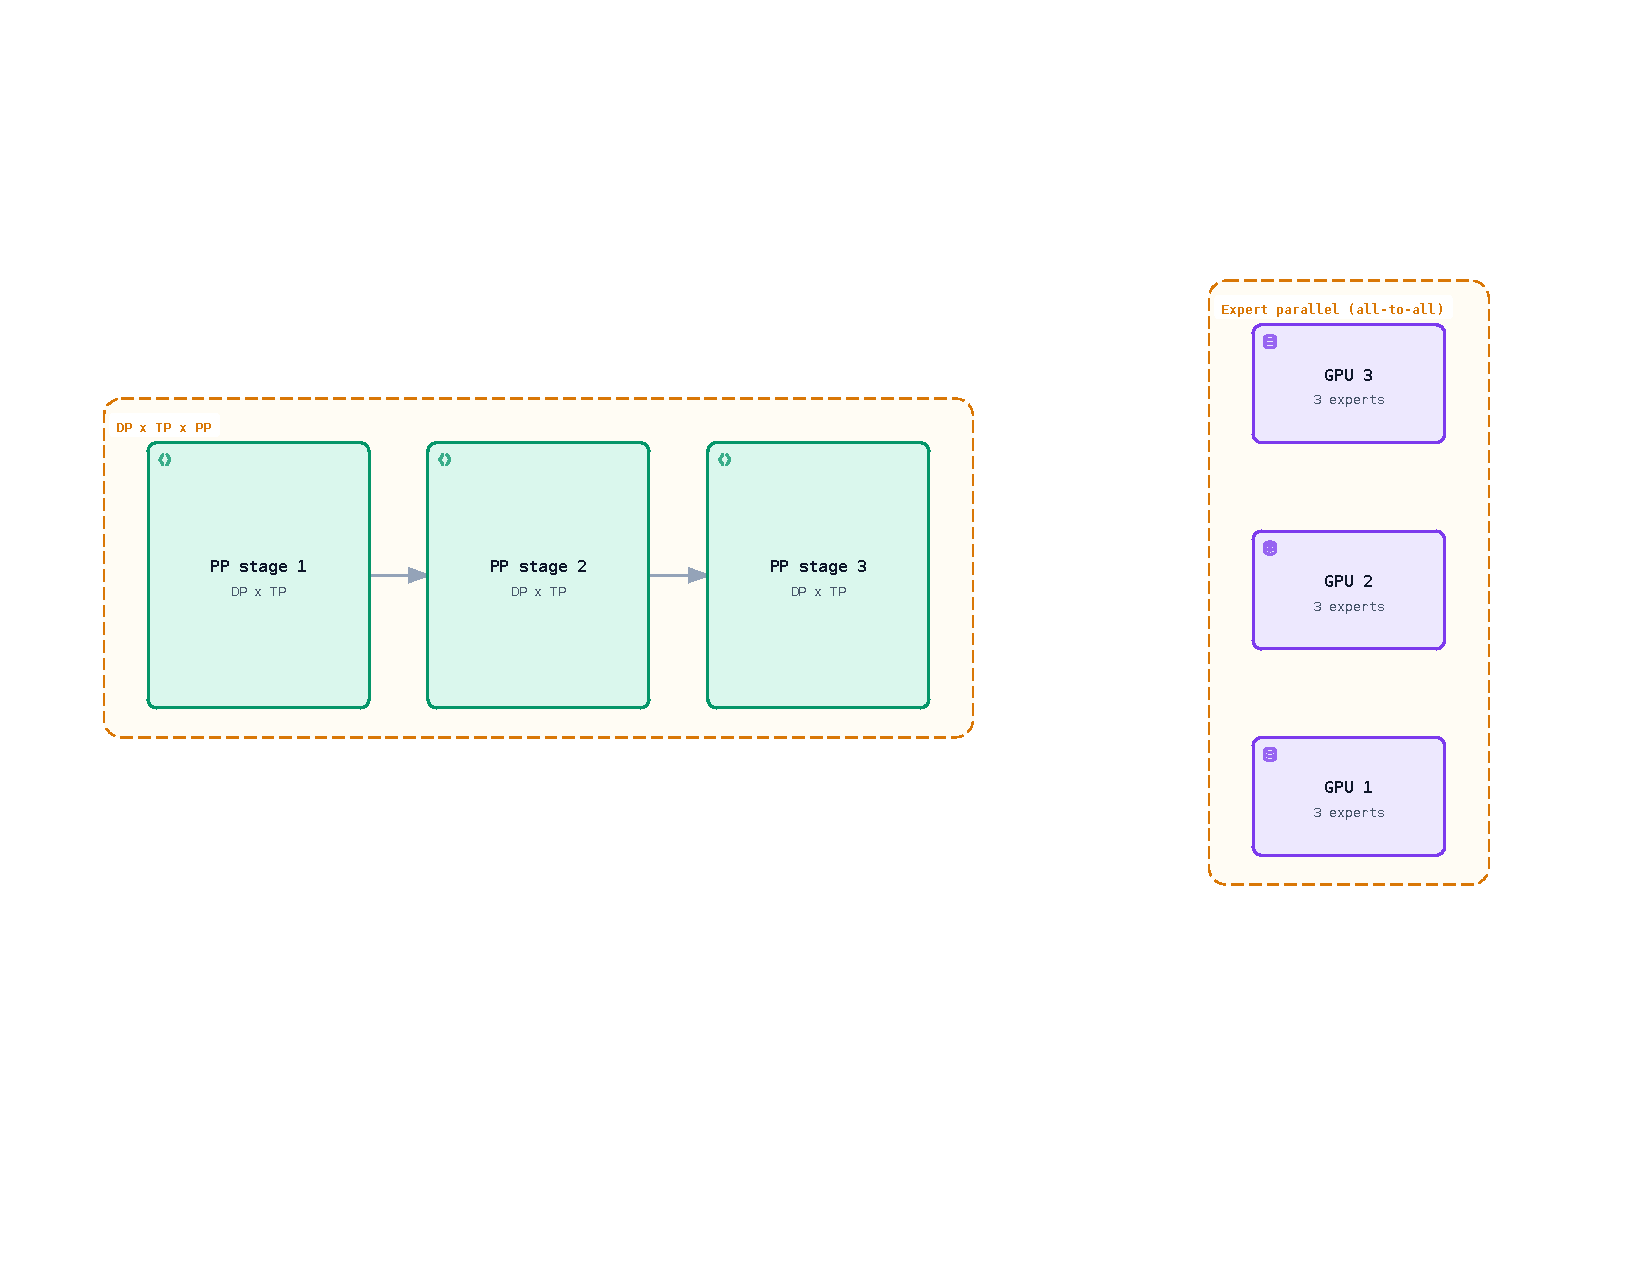
\includegraphics[keepaspectratio,alt={Fig 10.1 --- Composing the dimensions: each PP stage holds a DP replica, TP-sharded across GPUs; and EP's per-token all-to-all routes each token to the GPU holding its experts (ILLUSTRATIVE)},width=\maxwidth{\textwidth},keepaspectratio]{figures/fig-10-1002.pdf}}
\caption{Fig 10.1 --- Composing the dimensions: each PP stage holds a DP
replica, TP-sharded across GPUs; and EP's per-token all-to-all routes
each token to the GPU holding its experts (ILLUSTRATIVE)}

\label{fig:10.1}\end{figure}

\emph{\hyperref[fig:10.1]{Fig 10.1} --- The strategies are not either/or. Left: a DP × TP ×
PP stack --- the layer stack is cut into PP stages (green), each stage
is DP-replicated (orange) across nodes, and within a stage TP shards the
weights across 4 GPUs (blue). Right: expert parallel is a per-token
all-to-all --- each token may leave its home GPU to reach the GPU
holding its top-k experts. Which dimension binds determines which you
split first.}

\section{Mental Model}\label{mental-model}

Think of each strategy by \emph{what it trades bandwidth for}. Tensor
parallelism trades a lot of NVLink bandwidth to avoid duplicating
weights but adds per-layer sync. Pipeline parallelism trades low
bandwidth but accepts bubbles as the price of not holding all layers on
one GPU. Data parallelism trades gradient bandwidth (once per step) for
the convenience of replicated weights and is limited by having to fit
the whole model on each GPU.

The useful mental model is a \textbf{resource triangle}: we have weights
(memory), activations (work), and data (batch). Each strategy moves one
corner off a single GPU at the cost of communication. When a GPU runs
out of \emph{memory}, we reach for TP/PP (weight splitting). When a GPU
is \emph{idle} waiting, we reach for DP/CP (more work per GPU). When the
model is \emph{too big to replicate}, TP wins over DP. The binding
constraint chooses the strategy.

\subsubsection{\hyperref[tab:10.1]{Table 10-1} --- Parallelism strategies at a
glance}\label{table-10-1-parallelism-strategies-at-a-glance}

\begin{longtable}[]{@{}
  >{\raggedright\arraybackslash}p{0.2500\linewidth}
  >{\raggedright\arraybackslash}p{0.2500\linewidth}
  >{\raggedright\arraybackslash}p{0.2500\linewidth}
  >{\raggedright\arraybackslash}p{0.2500\linewidth}@{}}
\toprule\noalign{}
\begin{minipage}[b]{\linewidth}\raggedright
Strategy
\end{minipage} & \begin{minipage}[b]{\linewidth}\raggedright
What it splits
\end{minipage} & \begin{minipage}[b]{\linewidth}\raggedright
Communication need
\end{minipage} & \begin{minipage}[b]{\linewidth}\raggedright
Fits when
\end{minipage} \\
\midrule\noalign{}
\endhead
\bottomrule\noalign{}
\endlastfoot
Tensor (TP) & a layer's weights within a GPU group & high --- every
layer, over NVLink & model exceeds one GPU, fits a node \\
Pipeline (PP) & the layer stack into stages & low --- stage boundaries
only & model spans nodes \\
Data (DP) & the batch; replicates weights & gradient all-reduce per step
& model fits one GPU, need throughput \\
Expert (EP) & MoE experts; route-by-token all-to-all & high, per token &
MoE models \\
Sequence (CP) & the sequence/context dimension & medium & long contexts,
KV too big \\

\label{tab:10.1}\end{longtable}

\emph{(Strategies compose; the table names the primary cost each
trades.)}

\section{Worked Example}\label{worked-example}

\subsection{Why the Canonical 70B Doesn't Fit One
H100}\label{why-the-canonical-70b-doesnt-fit-one-h100}

The canonical model is 70B FP16 dense = 140 GB of weights {[}1P{]}
(reality check: 70 × 10⁹ params × 2 bytes). A single H100 has 80 GB of
HBM {[}2° FACT{]}. The arithmetic is immediate:

\begin{itemize}
\tightlist
\item
  The weights alone don't fit on one H100:
\end{itemize}

\[
140 \text{ GB weights} > 80 \text{ GB HBM}
\]

We need at least \(140 / 80 \approx 1.75\) → \textbf{≥ 2 GPUs just to
hold the weights} (and that's before KV cache, which adds
\textasciitilde2.5 MB/token at FP16 --- the 9.2K-token canonical prompt
needs \textasciitilde24 GB more). {[}2° DERIVED{]}

The canonical 8×H100 host (640 GB total) fits the weights + KV
comfortably, which is why the single-host baseline in earlier chapters
works. But if the model grows (say to 400B) or owns more, the split
becomes mandatory:

\subsection{Tensor Parallelism: Splitting Weights Across
GPUs}\label{tensor-parallelism-splitting-weights-across-gpus}

With tensor parallelism, the 140 GB weight is split across GPUs. On
2×H100: \(140 / 2 = 70\) GB per GPU, each now under the 80 GB ceiling.
But every transformer layer's matmuls now require an \textbf{all-reduce
of the layer's output across the TP group} --- a per-token, per-layer
exchange over NVLink. For the canonical 70B with \textasciitilde80
layers, that is \textasciitilde80 × tokens × output-size of
communication per forward pass. The all-reduce communication cost per
layer, per token is
\(T_\text{tp} = \text{tokens} \times n_\text{layers} \times \text{output-size} / B_\text{eff}\).
TP is only viable where the interconnect is very fast: on-node NVLink
(900 GB/s) keeps the sync cheap; over slow Ethernet it would drown.
{[}2° FACT{]}{[}2° DERIVED{]}

\subsection{Pipeline Parallelism: Splitting Layers, Accepting
Bubbles}\label{pipeline-parallelism-splitting-layers-accepting-bubbles}

Pipeline parallelism puts stage \(P\) on GPU \(P\). The cost is the
\textbf{pipeline bubble}: while the first micro-batch fills the pipeline
and the last one drains, stages sit idle. With \(P\) stages and \(m\)
micro-batches, the steady-state \textbf{ideal speedup} over a single
serial pass is:

\[
\text{ideal speedup} = \frac{m \cdot P}{m + P - 1}
\]

The \(P{-}1\) term in the denominator is the bubble: the pipeline fills
and drains exactly once per \(m\)-batch pass, so \(P{-}1\) stage-slots
are wasted out of the \(m \cdot P\) slots each stage would otherwise
work. With \(P = 4\) stages and \(m = 8\) micro-batches, ideal
utilization is

\[
\frac{8 \cdot 4}{8 + 4 - 1} = \frac{32}{11} \approx 2.9\times \quad (\text{out of } 4\times)
\]

--- a meaningful bubble. Fewer stages or more micro-batches shrink it:
with \(m = 32\),

\[
\frac{32 \cdot 4}{32 + 4 - 1} = \frac{128}{35} \approx 3.66\times.
\]

The lesson: PP is communication-light (each stage only moves activation
boundaries across the fabric) but always pays a bubble that grows with
stage count. {[}2° DERIVED{]}

\subsection{Data Parallelism: Replicating, Then Syncing
Gradients}\label{data-parallelism-replicating-then-syncing-gradients}

Data parallelism replicates the 140 GB model on every GPU. For the
gradient all-reduce: if the model has 140 GB × 2 (weights + gradients)
and we sync after each step across G GPUs, each GPU sends the full
gradient tensor once per step. The gradient bytes are

\[
\text{grad bytes} = 2 \times N \times \text{bytes/param} = 2 \times 70 \times 10^9 \times 4 \text{ B} \approx 280 \text{ GB}
\]

per step (BF16), and the sync time is
\(T = \text{bytes} / B_\text{eff}\). At 25 GB/s (single 200Gb/s link)
that is \texttt{280\ /\ 25\ ≈\ 11\ s} per step --- far too slow if the
step takes \textasciitilde1 s. At node NVLink 900 GB/s it is
\texttt{280/900\ ≈\ 0.31\ s}. The sync cost, not compute, often caps DP
at small scale unless the interconnect is fast. {[}2° DERIVED{]}

\section{Measurement}\label{measurement}

Four habits anchor the architect:

\begin{enumerate}
\def\labelenumi{\arabic{enumi}.}
\item
  \textbf{Measure weight residency before choosing a split.}
  \texttt{bytes\ =\ params\ ×\ bytes\_per\_param} lands first; it
  decides whether TP/PP (memory) or DP (replication) is even possible.
\item
  \textbf{Measure interconnect bandwidth where it matters.} H100 NVLink
  \textasciitilde900 GB/s per GPU is the on-node ceiling; cluster
  Ethernet/InfiniBand is 1--2 orders slower. Quote the number at the
  sync/frequency it will actually run.
\item
  \textbf{Measure the bubble and the step time.} For PP, log the
  fraction of idle GPU time (bubble) vs compute. For DP, time the
  gradient all-reduce as a fraction of step time --- if it exceeds
  \textasciitilde20\%, it caps scaling.
\item
  \textbf{Measure communication overlap.} The best systems overlap
  all-reduce with the next forward/backward compute. Log the
  non-overlapped comm time --- that is the true cost, not the raw bytes.
\end{enumerate}

\section{Common Mistakes}\label{common-mistakes}

\begin{itemize}
\item
  \textbf{Splitting with DP when the model doesn't fit.} DP replicates
  weights; if 140 GB \textgreater{} 80 GB, one DP replica doesn't even
  fit one GPU. Reach for TP/PP first.
\item
  \textbf{Using TP over a slow interconnect.} TP syncs every layer; over
  25 GB/s cluster fabric it bottleneck-cycles. TP belongs behind NVLink.
\item
  \textbf{Ignoring the pipeline bubble.} PP's idle stages waste real
  utilization; the bubble grows with stage count. It is not free.
\item
  \textbf{Quoting peak interconnect spec as sustained.} NVLink 900 GB/s
  is aggregate peak; real all-reduce achieves a fraction. Budget
  headroom.
\item
  \textbf{Treating parallelism as an either/or.} Real systems compose
  DP×TP×PP; the question is which dimension binds, not which one to use.
\end{itemize}

\section{Architecture Consequence}\label{architecture-consequence}

The parallelism strategy is forced by the binding constraint, and that
constraint is usually \textbf{memory} for large models:

\begin{itemize}
\item
  \textbf{A model that exceeds one GPU's memory} must split weights → TP
  (within a node, on NVLink) or PP (across nodes, low comm). Which one
  depends on whether the model fits a node: fits one node → TP among its
  GPUs; spans nodes → PP across them, with TP inside each node.
\item
  \textbf{A workload with high throughput demand} (like the canonical
  \textasciitilde10 rps / 40 rps) that fits one replicable model → DP to
  scale batch across GPUs, accepting the gradient-sync cost only if it
  trains/fine-tunes. For pure inference the canonical 70B fits one
  8×H100 node, so parallelism is often unnecessary at the single-host
  baseline.
\item
  \textbf{MoE models} (if chosen per Ch3) push toward EP, because only
  the active experts need residency per token.
\item
  \textbf{The canonical answer}: for the book's
  \textasciitilde70B/8×H100 scenario, no parallelism is required at the
  baseline; parallelism becomes the tool when the model or workload
  outgrows one node. The architect escalates through TP (in-node) → PP
  (cross-node) → DP (replicating a fitting model) in that order.
\end{itemize}

\begin{figure}
\centering
\pandocbounded{\includegraphics[keepaspectratio,alt={\hyperref[fig:10.2]{Fig 10.2} --- The five parallelization strategies and what each splits {[}ILLUSTRATIVE conceptual{]}},width=\maxwidth{\textwidth},keepaspectratio]{figures/fig-10-1001.pdf}}
\caption{\hyperref[fig:10.2]{Fig 10.2} --- The five parallelization strategies and what each
splits {[}ILLUSTRATIVE conceptual{]}}

\label{fig:10.2}\end{figure}

\emph{\hyperref[fig:10.2]{Fig 10.2} --- Tensor / pipeline / data / expert / sequence
parallelism, each drawn as its own object --- weight matrix, layer
stack, replicated model, MoE experts, context window --- splitting into
GPU shards beneath it.}

\section{What We Still Don't Know}\label{what-we-still-dont-know}

\begin{itemize}
\item
  \textbf{Optimal split for very large MoE or long-context models} is
  workload- and interconnect-dependent; the exact NVLink-vs-fabric
  crossover for a given model is {[}VERIFY{]}.
\item
  \textbf{2026 MoE scaling has moved the specialist/EP frontier.} Kimi
  K3 activates just 16 of 896 routed experts per token (2.8T total /
  104B active) via its Stable LatentMoE {[}1P: arXiv 2607.24653{]};
  Qwen3.8-Flash-Next routes 10+1 of 512 experts (125B total / 6B active)
  {[}1P: HF Qwen/Qwen3.8-Flash-Next{]}. These extreme sparsities (16/896
  ≈ 1.8\% expert activation) are why expert-parallel and fused
  cross-expert comm kernels (e.g.~MoE expert parallelism with fused
  compute/communication, as in DeepSeek's DeepEP/TileLang infra) are
  increasingly central to serving large MoE fleets {[}1P: arXiv
  2606.19348{]}. For the architect this changes the serving calculus: a
  frontier MoE's activated footprint (Kimi 104B, Qwen 6B) can be
  dramatically smaller than its total size, so the memory-bound EP
  decision must be made against \emph{active} parameters, not total.
\item
  \textbf{Communication-overlap efficiency} in real kernels is hard to
  predict from spec; sustained all-reduce throughput is {[}HYPOTHESIS{]}
  until measured on the target cluster.
\item
  \textbf{The right parallelism for mixed prefill/decode (P/D
  disaggregated) serving} --- where the prefill pool and decode pool may
  want different splits --- is an active research area and
  {[}HYPOTHESIS{]} for this book.
\end{itemize}

\section{End-of-Chapter Mini-Case}\label{end-of-chapter-mini-case}

An architect inherits a deployment where the internal Q\&A model (from
Ch1's mini-case) has been fine-tuned and grown to a 400B-parameter MoE.
The team reports ``parallelism is killing us --- everything is slow.''
The architect applies this chapter's lens. First, weight residency: a
400B model needs
\textasciitilde{}\texttt{400e9\ ×\ 2\ bytes\ =\ 800\ GB} even before KV
--- it spans \textasciitilde11×H100 at minimum, far beyond one node. It
does not fit a node, so pure TP can't span it; PP across nodes is
required. Within each node, the MoE active weights are small, so the
team uses EP to shard experts + TP inside the node. The architect
measures the interconnect: the cross-node PP boundary runs over the
cluster fabric (not NVLink), so they minimize the number of PP stages to
shrink the bubble, and they verify the DP gradient-sync (if fine-tuning)
stays under \textasciitilde20\% of step time. The result: a composed PP
× EP × TP configuration whose binding constraints (memory across nodes +
expert routing) are each addressed by the strategy that trades the right
bandwidth. The team's ``parallelism is slow'' becomes a precise,
diagnosed, and fixed split.
